In this section, we discuss the application of QC-extraction to achieve the performance of cryptographic models such as noisy storage models. We will mainly focus on two applications of QC-extractors. First, QC-extractor gives rise to entropic uncertainty relations with quantum side information, and second noisy storage model; in other words, any two-party cryptographic protocol can be implemented securely as long as the adversary’s storage device has sufficiently low quantum capacity.  

\subsection{Entropic uncertainty relations with quantum side information}
% \%\%\% \textcolor{red}{This paragraph gives ideas about uncertainty principle of physics.}
The uncertainty principle is one of the fundamental theories of quantum mechanics. 
Uncertainty relations, originally proposed by Heisenberg $\Delta x \Delta p \geq \frac{h}{4\pi}$, is one of the most prominent examples that show how quantum mechanics differs from the classical world. Perhaps, the best known in the form given by Robertson \cite{robertson1929uncertainty}, who extended Heisenberg's result to two arbitrary observables \footnote{In quantum physics, an observable is a physical quantity that can be measured, for example, position and momentum.} $A$ and $B$. Uncertainty relation states that if we prepare many copies of the state $\ket{\psi}$, and measure each copy individually using either observable $A$ or $B$, we have 
\[\Delta A \Delta B \geq \frac{1}{2} |\bra{\psi}[A,B]\ket{\psi}|\]
where $\Delta X = \sqrt{\bra{\psi}X^2\ket{\psi} - \bra{\psi}X\ket{\psi} }$ for $X = A, B$ is the standard deviation resulting from measuring $\ket{\psi}$ with observable $X$. This means that there is no way to simultaneously specify definite values of non-commuting\footnote{Two observables $A$ and $B$ are said to be commuting if $AB = BA$, thus, commutator $[A,B] = 0$,  where $ [A,B] = AB-BA$.} observables with great precision. 

% section IV of paper

Entropic uncertainty relations provide a contemporary way to express the notion of uncertainty in quantum mechanics. It has interesting applications in quantum cryptography, the entropic uncertainty relations allow to provide the security proof of cryptographic protocols.  Briefly, it provides a subtle interplay between uncertainty and entanglement.  We consider a bipartite guessing game, which consist of Alice and Eve, to understand the  entropic uncertainty relations. Entropic uncertainty relation allows us if Eve can or cannot predict the outcomes of two non-commuting measurements performed on Alice’s state.

% section 3.4 of https://ocw.tudelft.nl/wp-content/uploads/LN_Week3.pdf

Assume Eve only has classical memory, i.e., she might make measurements on the qubits during the transmission, but she cannot keep any entanglement with herself. This is equivalent to Eve preparing Alice’s qubits herself. We now define the \textit{guessing game} below:

\begin{tcolorbox}
    {\bf Guessing Game:}
    \begin{enumerate}
        \item {\bf Eve:} Prepares a qubit $\rho_{A}$ and sends it to Alice
        \item {\bf Alice:} Chooses a random bit $\Theta \in \{0, 1\}$
        \item {\bf Alice:} If $\Theta = 0$, then Alice measures $\rho_{A}$ in the computational basis,  i.e., $\set{\ket{0},\ket{1}}$; otherwise, she measures $\rho_{A}$ in the Hadamard basis,  i.e., $\set{\ket{+},\ket{-}}$
        \item {\bf Alice:} Records the measurement outcome $X \in \{0, 1\}$
        \item {\bf Alice:} Announces $\Theta$
        \item {\bf Eve:} Wins if she correctly guesses $X$
    \end{enumerate}
\end{tcolorbox}
\begin{figure}
    \centering
    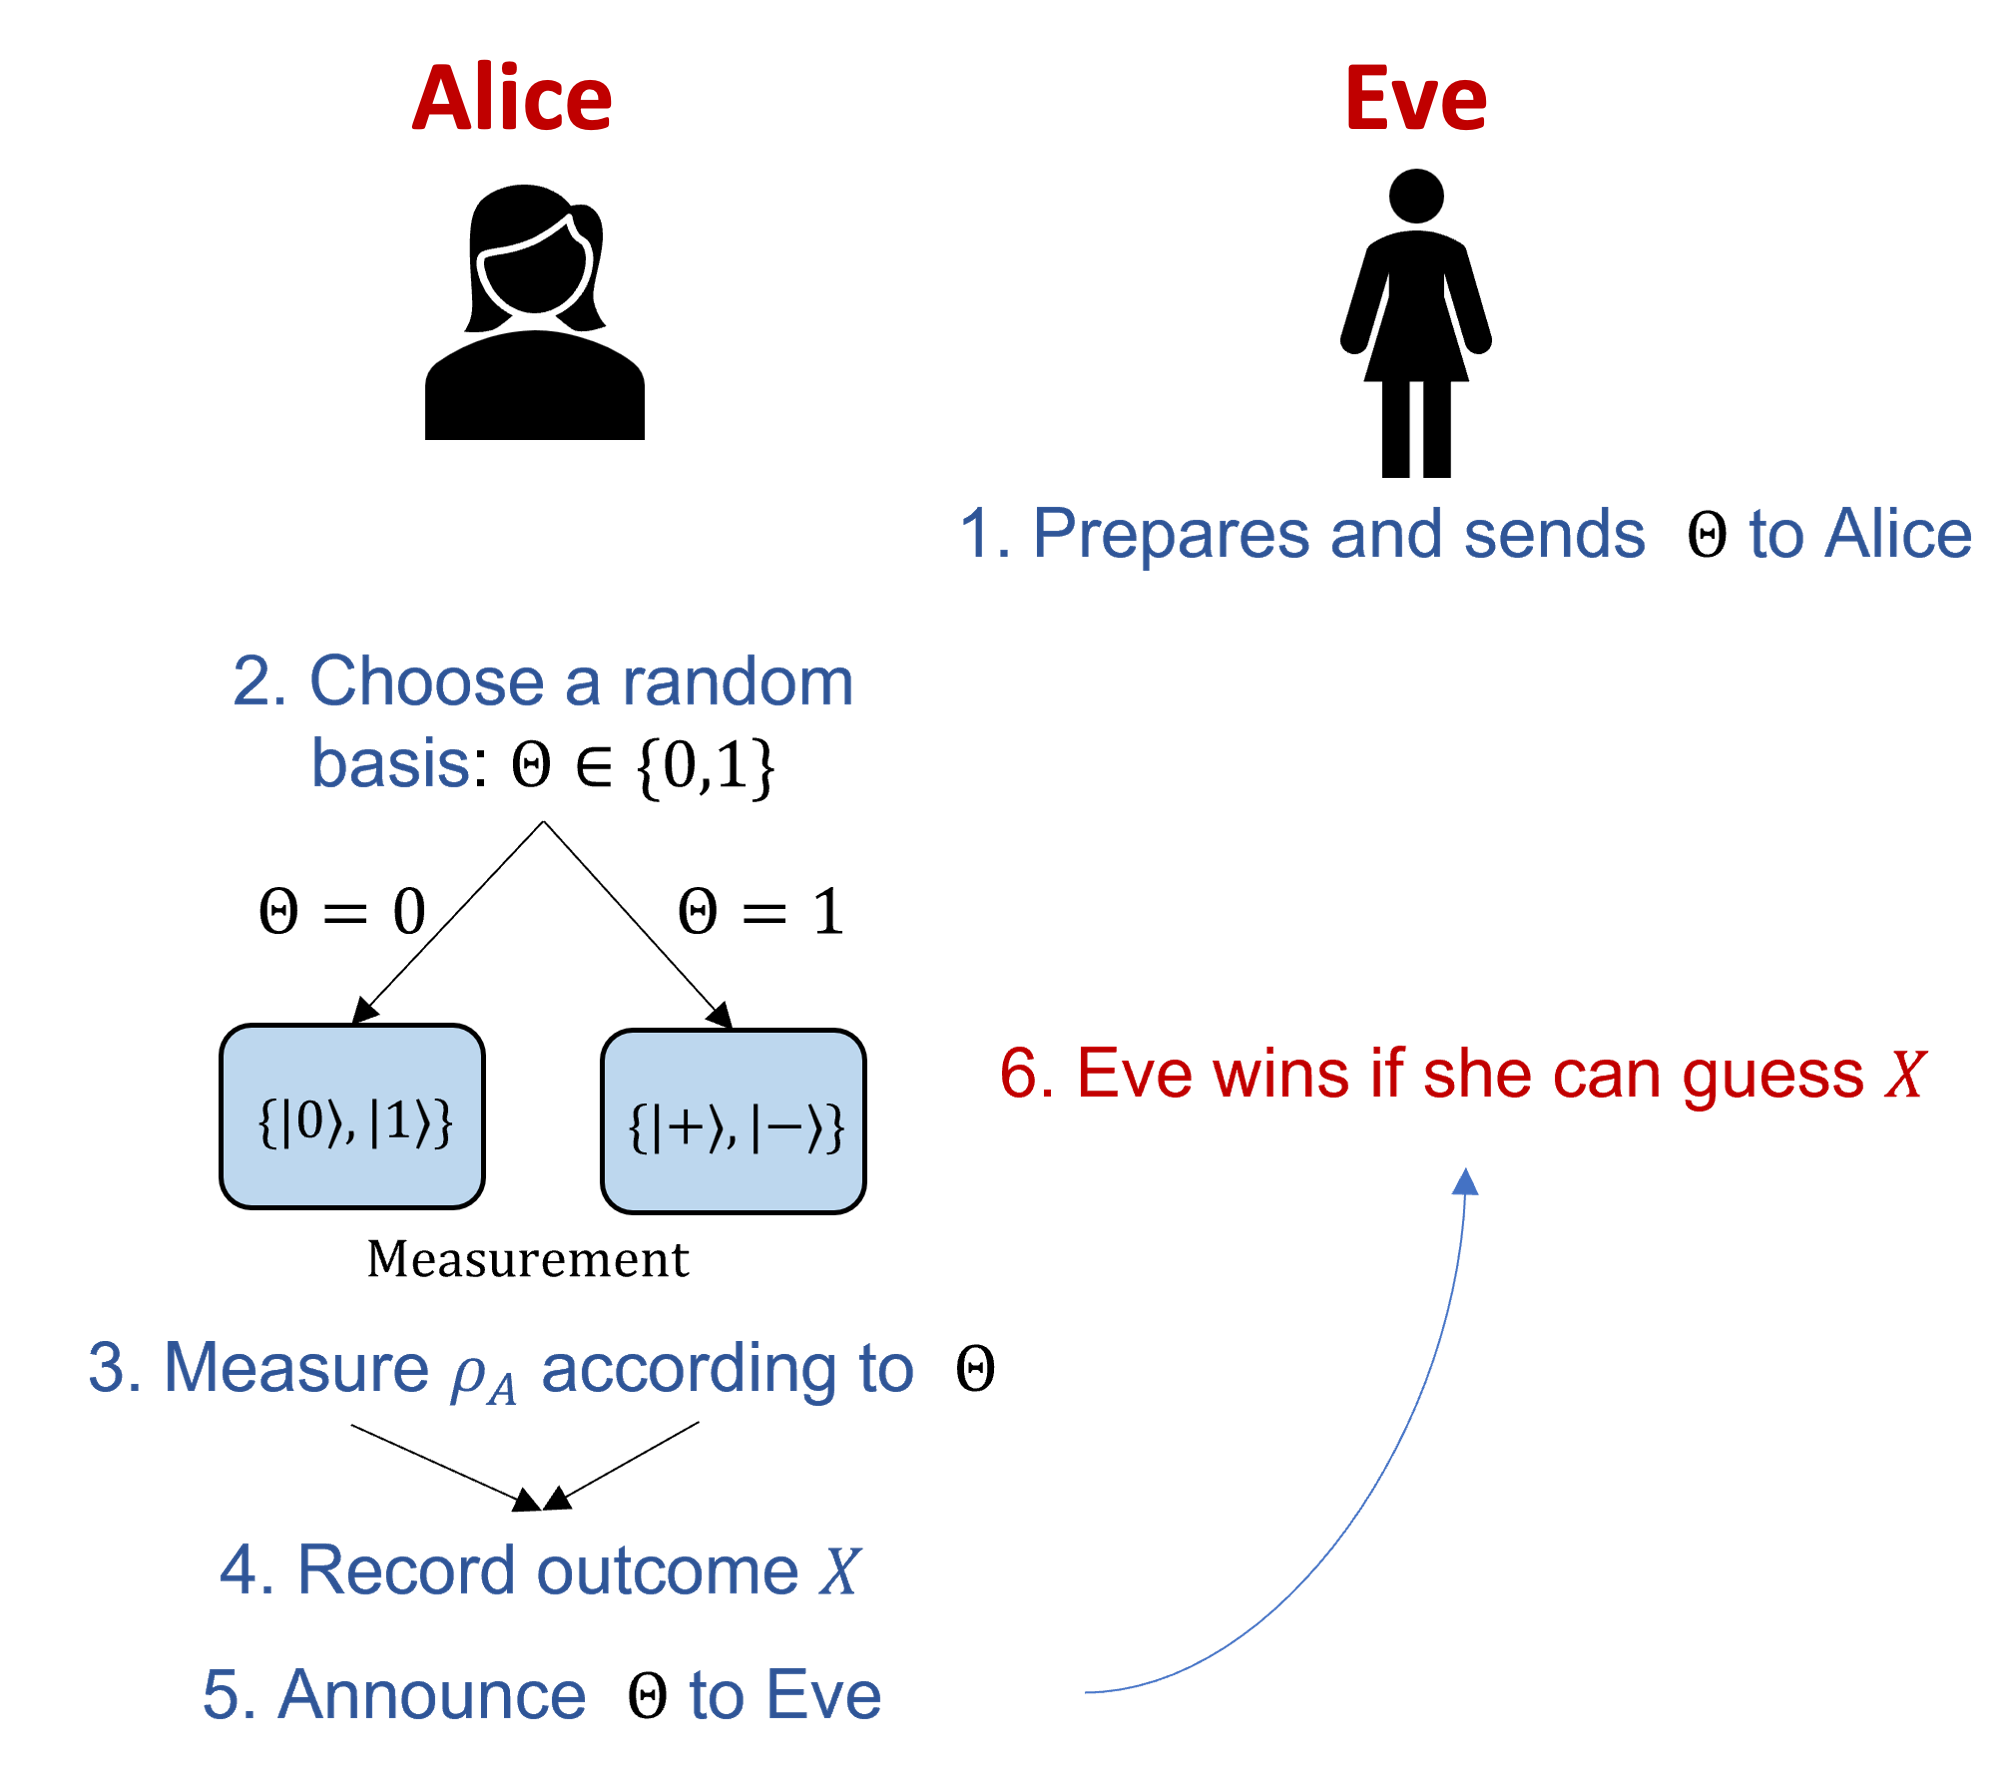
\includegraphics[scale=0.5]{Images/uncertainty.png}
    \caption{The bipartite guessing game between Alice and Eve.}
    \label{fig:uncertainty}
\end{figure}
\autoref{fig:uncertainty} summarizes the guessing game defined above. The objective is to make sure that Eve cannot fully predict Alice’s measurement outcome. Consider the following example, where the joint state between Alice and Eve is 
\begin{align*}
    \rho_{A E} 
    &= \ket{0} \bra{0}_{A} \otimes \rho_{E},
\end{align*}
where Alice measures system $A$ in either the computational or the Hadamard basis to obtain the secret key. 
To see why this captures the essence of the uncertainty principle, note that if the measurements are non-commuting, then there exists no state $\rho_{A}$ that Eve can prepare, which would allow her to guess the outcome for both choices of measurements with certainty. Uncertainty can be understand as  a bound on the average probability that Eve correctly guesses $X$:
\begin{align*}
    \Pr[X \mid \Theta] 
    &= \Pr[\Theta = 0] \cdot \Pr[X \mid \Theta = 0] + 
    \Pr[\Theta = 1] \cdot \Pr[X \mid \Theta = 1] \\
    &= \frac{1}{2} [\Pr[X \mid \Theta = 0] + \Pr[X \mid \Theta = 1]\le \epsilon,
\end{align*}
where the second equality holds if Alice chooses her measurement basis $\Theta$ at random, i.e. with uniform probability $1 / 2$ for each option. In the case where Eve holds no additional information except for the basis where Alice has performed the measurement, it can be shown that $\epsilon < 1$. To understand this, suppose Eve always aims to correctly guess $X$ regardless of whether $\Theta = 0$ or $\Theta = 1$. Then she requires $\Pr[X \mid \Theta = 0] = 1$, i.e. she should prepare a state that will always produce a deterministic outcome when Alice measures in the computational basis. In order for this to happen, Eve can send the state $\ket{0} \bra{0}_{A}$, where Alice, upon measuring in the computational basis, will always produce $X = 0$. However, if Eve has used the strategy of preparing $\ket{0} \bra{0}_{A}$ and Alice measures in the Hadamard basis, then
\begin{align*}
    \Pr[X \mid \Theta = 1] 
    &= \max\{\Pr[X = 0 \mid \Theta = 1], \Pr[X = 1 \mid \Theta = 1] \\
    &= \max\{\Tr[\ket{+} \bra{+} \ket{0} \bra{0}], \Tr[\ket{-} \bra{-} \ket{0} \bra{0}]\}= \frac{1}{2}. 
\end{align*}
Thus, if Eve uses this strategy of preparing $\rho_{A} = \ket{0} \bra{0}_{A}$ in order to guess Alice’s outcome $X$, then whenever $\Theta = 1$, this corresponds only to a random guess. So, in this protocol, since Eve does not know beforehand what basis Alice will choose to measure in, she has to prepare a state that will maximize her guessing probability in both cases of Alice measuring in the standard basis, and also the Hadamard basis. The above example shows that this guessing probability can never be equal to $1$.

Note that in order for Eve to maximize the guessing probability $\Pr[X \mid \Theta]$ over $\rho_{A}$, without loss of generality, we consider the outcome to be $X = 0$,
\begin{align*}
    \Pr[X \mid \Theta] 
    &= \frac{1}{2} (\Tr[\rho_{A} \ket{0} \bra{0}] + \Tr[\rho_{A} \ket{+} \bra{+}])= \frac{1}{2} \Tr[\rho_{A} (\ket{0} \bra{0} + \ket{+} \bra{+})]
\end{align*}
then she has to prepare $\rho_{A}$ in the pure state corresponding to the eigenvector of $\ket{0} \bra{0} + \ket{+} \bra{+}$ with the largest eigenvalue, which is $\lambda_{\max} 
    = 1 + {1/\sqrt{2}}.$
% \begin{align*}
%     \lambda_{\max} 
%     &= 1 + \frac{1}{\sqrt{2}}.
% \end{align*}
Therefore,
\begin{align*}
    \Pr[X |\Theta] 
    &= \frac{1}{2} + \frac{1}{2 \sqrt{2}} 
    < 1.
\end{align*}

To calculate Eve's guessing probability, we write a quantum state in the following form \cite{wilde2013quantum,nielsen2002quantum}:
\begin{align*}
    \rho_{A} 
    &= \frac{1}{2} (\I + v_{x} X + v_{y} Y + v_{z} Z)
\end{align*}
for a vector $v = (v_{x}, v_{y}, v_{z})$. Then,
\begin{align*}
    &\Tr[\rho_{A} \ket{0} \bra{0}] 
    = \frac{1}{2} (1 + v_{z}), 
    &\Tr[\rho_{A} \ket{1} \bra{1}] 
    = \frac{1}{2} (1 - v_{z}), \\
    &\Tr[\rho_{A} \ket{+} \bra{+}] 
    = \frac{1}{2} (1 + v_{x}), 
    &\Tr[\rho_{A} \ket{-} \bra{-}] 
    = \frac{1}{2} (1 - v_{x}). 
\end{align*}
\begin{align*}
    \text{Also, } \Pr[X \mid \Theta] 
    &= \frac{1}{2} \max\{\Tr[\rho_{A} \ket{0} \bra{0}], \Tr[\rho_{A} \ket{1} \bra{1}]\} + 
    \frac{1}{2} \max\{\Tr[\rho_{A} \ket{+} \bra{+}], \Tr[\rho_{A} \ket{-} \bra{-}]\}
\end{align*}
maximized over all possible states $\rho_{A}$. Since the maximizations of both expression are symmetric around $v_{z} = 0, v_{x} = 0$, respectively.  Consider only the case where $v_{z}, v_{x} \ge 0$. Thus, we get,
\begin{align*}
    \Pr[X \mid \Theta]_{\rho_{A}} 
    &= \frac{1}{2} \Tr[\rho_{A} (\ket{0} \bra{0} + \ket{+} \bra{+})] = \frac{1}{4} (2 + v_{x} + v_{z}), \qquad v_{x}^{2} + v_{z}^{2} \le 1.
\end{align*}
Note that the maximum occurs when $v_{x}^{2} + v_{z}^{2} = 1$. 
% Letting $v_{x} = \cos(t)$, $v_{z} = \sin(t)$ gives that
% \begin{align*}
%     \max_{t} \{\cos(t) + \sin(t)\}
% \end{align*}
% obtained for $\cos(t) = \sin(t) = 1 / \sqrt{2}$. 
Therefore, by the change of variable as  $v_{x} = \cos(t)$, $v_{z} = \sin(t)$, we get,  the probability of Eve winning the game is 
\begin{align*}
    \Pr[X \mid \Theta]_{\rho_{A}} 
    &= \frac{1}{2} + \frac{1}{2 \sqrt{2}} 
    \approx 0.85.
\end{align*}
In a more general scenario, Eve may even have classical information about $\rho_{A}$. Following the same steps as above, we can show that 
\begin{align*}
    \Pr[X | \Theta C]_{\rho_{AC}} 
    &= \frac{1}{2} + \frac{1}{2 \sqrt{2}} 
    \approx 0.85.
\end{align*}
Thus, the min-entropy $\Hmin(X \mid \Theta C) = - \log \Pr[X \mid \Theta C] \approx 0.22$. 

If we always allow Eve maximum information about everything, she may prepare a larger state $\rho_{AE}$,  i.e., Eve also holds the purification and send the $\rho_A$ to Alice.  Then one can show that if Eve can be entangled with Alice’s qubit, then she can guess perfectly.

Finally, if we want to keep $X$ secret from Eve, we need to use two aspects of quantum mechanics:
\begin{enumerate}
    \item Uncertainty: If Eve has no (or little) entanglement with Alice, then she cannot certainly predict the outcomes of two non-commuting measurements. So it is difficult to guess Alice’s measurement outcomes, i.e., $\Pr[X | E \Theta] < 1$, or equivalently, $\Hmin(X | E \Theta) > 0$.
    \item Entanglement: We need to ensure there exists some entanglement between Alice and Eve. For this, we can use the fact that entanglement is \textit{monogamous} \footnote{Please see the page on Wikipedia \href{https://en.wikipedia.org/wiki/Monogamy_of_entanglement}{Monogamy of entanglement}}, that is if we find a large amount of entanglement between Alice and Bob, then we know that Eve has very little entanglement with either Alice or Bob, and therefore the min-entropy should be large. Hence, Eve cannot guess the outcome of Alice, and entropic uncertainty ensures security!
\end{enumerate}

% https://ocw.tudelft.nl/course-lectures/3-4-1-uncertainty-principles-simple-version-bb84/
% table on page 17


Below, in \autoref{tab:lower_bounds}, we summarize the various methods used for constructing QC-extractions to achieve the uncertainty relations for the min-entropy \cite{berta2013quantum,Berta_2014}:

\begin{table}[h]
    \centering
    \begin{tabular}{|l|c|}
        \hline
         & Lower bounds for smooth conditional min-entropy $\Hmin$ \\
        \hline 
        Unitary $2$-design & $\log |A| + \Hmin^{\delta}(A | E)_{\rho} - \log\left(\frac{1}{(\varepsilon^{2} / 2 - 2 \delta)^{2}}\right)$ \\
        \hline
        Almost unitary $2$-design & $\log |A| + \Hmin^{\delta}(A | E)_{\rho} - \log\left(\frac{1}{(\varepsilon^{2} / 2 - 2 \delta)^{2}}\right) - \log(1 + \zeta)$ \\
        \hline
        All $|A| + 1$ MUBs & $\log(|A| + 1) + \Hmin^{\delta}(A | E)_{\rho} - \log\left(\frac{1}{(\varepsilon^{2} / 2 - 2 \delta)^{2}}\right)$ \\
        \hline
        Single qudit MUBs & $n (\log(d + 1) - 1) + \min\left\{0, \Hmin^{\delta}(A | E)_{\rho} - \log\left(\frac{2}{\delta'^{2}} + \frac{1}{1 - 2 \delta}\right)\right\}$ \\
        & \hfill $ - \log\left(\frac{1}{(\varepsilon^{2} / 2 - 2 \delta - \delta')^{2}}\right) - 1$\\
        \hline
    \end{tabular}
    \vspace{5pt}
    \caption{Entropic uncertainty relations with quantum side information for the smooth conditional min-entropy for approximation parameters $\varepsilon > 0$, $\zeta \ge 0$, $\delta \ge 0$, and $\delta' > 0$.}
    \label{tab:lower_bounds}
\end{table}

\subsection{Noisy-Storage Model}

Quantum computer benefits computing resources for those algorithms with computational assumptions, but a drawback is that the security can be broken retroactively. Most two-party protocols that have been executed to date will lose their security because the adversary can use the quantum computer to break the protocol. One way to solve this problem is to consider physical assumptions rather than computational assumptions. The most straightforward one is storage. 

In classical cryptography, physical assumptions are usually made as the \emph{bounded-storage model}, which assumes that the adversary can only store a certain number of classical bits. After introducing quantum communication, one now assumes that the adversary's quantum storage is limited to a certain number of qubits but no restriction on the classical bits. This is known as \emph{bounded-quantum-storage model}. More generally, one can also invoke the noisy storage model, where the quantum storage is not only bounded but also noisy in general \cite{tudelftQC}, to incorporate both the amount of storage and noise. \cite{Konig_2012} introduced the concept of a \emph{noisy-storage model}.

\begin{definition}\textbf{(Noisy Quantum Memory)}
Given a device whose input states are in some Hilbert space $\mathcal{H}_{in}$, a \emph{noisy quantum memory} is a state $\rho$ stored in the device decoheres over time. That is, the content of the memory after some time $t$ is a state $\mathcal{F}_t(\rho)$, where $\mathcal{F}_t : \mathcal{H}_{in} \rightarrow \mathcal{H}_{out}$ is a completely positive trace-preserving map corresponding to the noise in the memory.

Considering the security, the intuition is that security is possible as long as the amount of information that the adversary can store in his memory device is limited. Therefore, the central assumption of the model is that during waiting times $\delta t$ introduced into the protocol, the adversary can only store quantum information using a limited and unreliable quantum memory device. In particular, the adversary can store an unlimited amount of classical information while also doing any operation at the moment. That means he is able to use any encoding and decoding operations before and after using his memory device. Notice that the input spaces can be in the form of $\mathcal{H}_{in} = (\C^d)^{\otimes N}$ and channels $\mathcal{F} = \mathcal{N}^{\otimes N}$ with $\mathcal{N}: \mathcal{H}_{in} \rightarrow \mathcal{H}_{out}$.

To analyze the security of a noisy-storage model, we first introduce a technique called \emph{weak string ensure}.

\begin{definition}\textbf{(Weak String Erasure)}
In a two-party secure computation, \emph{weak string erasure} is a primitive that provides Alice with a random bit string $X^n \in \{0,1\}^n$ and Bob with a randomly chosen substring $X_{\mathcal{I} = (X_{i_1}, X_{i_2}, \dots, X_{i_r})}$ together with index set $\mathcal{I} = \{i_1, i_2, \dots, i_r\}$ specifying the location of these bits \cite{Konig_2012}.
\end{definition}

The motivation behind the primitive weak string erasure was to create a basic quantum protocol that builds up classical correlations between Alice and Bob which are later used to implement more interesting cryptographic primitives. We can construct a very simple protocol for weak string erasure and prove its security using a bitwise QC-randomness extractor.

The protocol is basically the same as the one provided in \cite{Konig_2012}, but in our case, instead of using only 2 MUBs per qubit, there will be 3. The procedure is as follows: 
\begin{tcolorbox}
\textbf{Protocol Weak String Erasure (WSE):} 
\newline
\textbf{Output: }$x^n \in \{0,1\}^n$ \textbf{to Alice,} $(\mathcal{I, |z|^{\mathcal{I}}}) \in 2^{[n]} \times \{0,1\}^{\mathcal{I}}$ \textbf{to Bob.}
\\ \hspace*{\fill} \\
\hspace*{0.5cm} \textbf{1. Alice:} Creates $n$ EPR-pairs $\Phi$, and sends half of each pair to Bob.
\newline
\hspace*{0.5cm} \textbf{2. Alice:} Chooses a bases-specifying string $\theta^n \in_R \{0,1,2\}^n$ uniformly at random. 
\newline
\hspace*{1cm} For all $i$, she measures the $i$-th qubit in the basis $\theta_i$ to obtain outcome $x_i$.
\newline
\hspace*{0.5cm} \textbf{3. Bob: } Chooses a basis string $\tilde{\theta}_i \in_R \{0,1,2\}^n$ uniformly at random. When 
\newline
\hspace*{1cm} receiving the $i$-th qubit, Bob measures it in the basis of $\tilde{\theta}^n$ to obtain outcome $\tilde{x}_i$.
\\ \hspace*{\fill} \\
Both parties wait time $\Delta t$. 
\\ \hspace*{\fill} \\
\hspace*{0.5cm} \textbf{4. Alice: } Sends the basis information $\theta^n$ to Bob and outputs $x^n$.
\newline
\hspace*{0.5cm} \textbf{5. Bob: } Computes $\mathcal{I} = \{i \in [n] | \theta_i = \tilde{\theta}_i\}$, and outputs $(\mathcal{I, |z|^{\mathcal{I}}}) := (\mathcal{I}, \tilde{x}_{\mathcal{I}})$.
\end{tcolorbox}

The proof of the correctness of the protocol and in regards to a dishonest Alice can be found in \cite{Konig_2012}. To prove the security against a dishonest Bob, we first consider the general form that any attack on Bob takes in the \autoref{fig:nsm2}.

\begin{figure}[!htb]
    \centering
    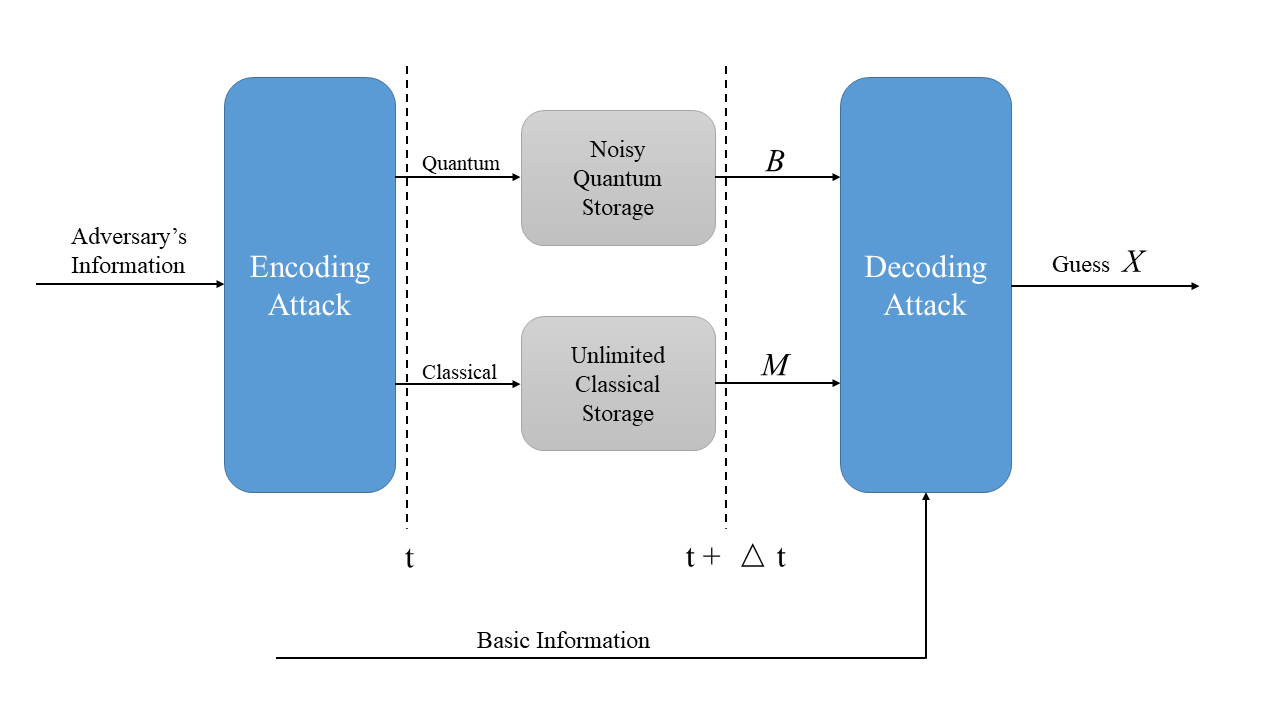
\includegraphics[scale=0.37]{Images/NSM2.png}
    \caption{Any attack of dishonest Bob is described by an encoding attack $E$ and a ‘guessing’ attack.}
     \label{fig:nsm2}
\end{figure}
% \newline
% \newline

Note that the noisy-storage model only assumes that Bob has to use his storage device during waiting times $\delta t$, which means when attacking the protocol above, he can store the incoming qubits perfectly until $n$ qubits arrive. Let $\mathcal{Q}$ denote Bob’s quantum register containing all $n$ qubits. Since there is no communication between Alice and Bob during the transmission of these n qubits, we can assume that Bob first waits for all n qubits to arrive before mounting any form of attack. Besides, as any operation in quantum theory is a quantum channel, Bob’s attack can be described by a quantum channel $\mathcal{E}: \mathcal{S}_{\leq}(\mathcal{Q}) \rightarrow \mathcal{S}_{\leq}(\mathcal{H}_{in} \otimes M)$, where this map takes $\mathcal{Q}$ to some quantum state on the input of Bob's storage device, $\mathcal{H}_{in}$, and $M$, some arbitrarily large amount of classical information. For example, $\mathcal{E}$ could be an encoding into an error-correcting code. 

Then, by the assumption of the noisy-storage model, Bob’s quantum memory is then affected by noise $\mathcal{F}: \mathcal{S}_{\leq}(\mathcal{H}_{in}) \rightarrow \mathcal{S}_{\leq}(\mathcal{H}_{out})$. After the waiting time, the joint state held by Alice and Bob in the purified version of the protocol (i.e., before Alice measures) is thus of the form

$$\rho_{ABM} = \mathcal{I}_A \otimes [(\mathcal{F} \otimes \mathcal{I}_M) \circ \mathcal{E}](\Phi^{\otimes n})$$

where $\Phi$ is an EPR-pair. And after the waiting time, Bob can perform any form of quantum operation to try and recover information from the storage device. Note that, in principle, Bob’s goal is to recover $X$ alone, for which he could potentially use his basis information $\Theta$. In fact, we can ignore the basis information in the analysis. That is, we only need to analyze decoding maps $\mathcal{D}: \mathcal{S}_{\leq}(\mathcal{H}_{in} \otimes M) \rightarrow \mathcal{S}_{\leq}(\mathcal{Q})$ trying to recover the initial entanglement between Alice and Bob.

After implementing the task of `Weak String Erasure' as above, we consider the usage of bitwise QC-extrators as linking security to the entanglement fidelity (quantum capacity) of the noisy quantum storage. Earlier, we came across the fact that one of the desirable properties of a bitwise QC-extrator is that, in addition to its computational efficiency, we observe that the unitaries act on single qubits. So, by changing the encoding from a qubit scheme to a qubit six-state scheme, we use the bitwise QC-extrator, defined in Theorem \ref{theorem:bitwiseqc}. This gives us a strong converse classical capacity replaced by the strong converse quantum capacity. This then extends the parameter regime where the security of all existing protocols can be proven.  Even though there is in general, no closed expression for the strong converse quantum capacity, we can calculate security rates by means of the entanglement cost of quantum channels, which is an upper bound on the strong converse quantum capacity. As a brief overview, the entanglement cost of a quantum channel is the minimal rate at which entanglement (between sender and receiver) is needed in order to simulate many copies of a quantum channel in the presence of free classical communication.
\end{definition}